\documentclass[output=paper,modfonts,nonflat]{langsci/langscibook} 

\title{Givenness marking in a mixed system: Constituent order vs. determiners} 
\author{Alexandra Simonenko\affiliation{Research Foundation Flanders \& Ghent University}\lastand Anna Carlier\affiliation{Université de Lille}}
% \chapterDOI{} %will be filled in at production

% \epigram{}

\abstract{This paper investigates the interaction between constituent order and the use of determiners as means of marking givenness, understood here as a non-presuppositional existential inference that arises as a result of interpreting a predicate with respect to a context-specified situation, in light of (a version of) *New $\succ$ Given principle of \citet{Kucerova:2012}. We attribute the principle to how situation binding operates in clauses, instead of postulating a presupposition-introducing operator and test it on new quantitative data from Medieval French, a system employing both determiners and constituent order for information structuring. Our results show that the constraint in question is respected across the board except for the cases when it is obviated by the presence of a morphological trigger of existential presupposition. We also show that a game-theoretic simulation incorporating this constraint matches very closely historical French data.}

%ADD BibTex Engine biber
%ADD Steiner 2014 on V2 and Information Structure

\begin{document}

\maketitle
\section{Introduction} 

This chapter focuses on the interactions between determiner types and constituent order in the marking of givenness in the history of French, on the basis of data from the twelfth to the seventeenth century. We understand givenness here in a weak sense of an existential inference that emerges when a nominal predicate is interpreted relative to a particular, discourse-specified situation. Medieval French is commonly assumed to have employed syntactic means for the expression of information structure. Because of the absence of native speaker judgements and speech recordings for historical data, identifying the exact information structural import of syntactic configurations no longer available in Modern French, such as the clause with a preverbal object in (\ref{ov1}), is a complex task. However, the consensus states that the variable placement of arguments had mostly to do with the way their denotation related to the contextual information.

\ea \label{ov1}
\gll Iceles miracles vit li pelerins\\
 these miracles saw the pilgrim\\
\glt ``The pilgrim saw these miracles'' \hfill \tiny{(1210-BORON-PENN-P,32.441)}\label{ex:ovs}
\z

%Likewise, \citet[61]{LabelleHirschbuhler:2005} argue that the preverbal position hosted either topicalized or focalized constituents. 

%cite Zimmermann 2014 who says that XP in V2 is a focus (cited by Larrivee)
%Ingham (2018a)

\citet{MarchelloNizia:1995}, who was among the first to investigate the tendency of Old French to have the verb immediately follow the first constituent (i.e. the so called V2-order, explored in a long series of works starting with \citet{Skarup:1975}), suggested that the first preverbal position was reserved for elements establishing a link with the previous discourse (for a similar intuition in \citet{Vennemann:1974} and \citet{Harris:1978}). \citet[117]{RinkeMeisel:2009} argue that ``the pre-verbal position correlates with a topic-interpretation and the post-verbal position with a non-topic interpretation''. \citet[24]{KaiserZimmermann:2011} propose that ``the positioning of one or more non-subject constituents to the left of the finite verb in declarative root clauses directly correlates with their discourse status, i.e. with their interpretation as either topicalized or focalized constituents''. They assume a split CP involving Topic and Focus projections. Based on an extensive corpus data analysis, \citet{LabelleHirschbuhler:2018} conclude that although the distribution is not categorical, the initial constituent in V2 configurations tend to be topical. V2 with non-subject preverbal constituents progressively becomes more rare until the constituent order in declarative sentences effectively converges onto SVO.

%For instance, they analyze the preverbal direct object in (\ref{qlr}) as focalized in the sense of ``special attention [being] drawn'' to this constituent, ``irrespective of the fact that it may constitute new information or information already given in the previous linguistic context''.

%\ea \label{qlr}
%\gll Un altre adversarie li suscitad nostre Seignur\\
%a other adversary him raised-up our Lord \\
%\glt `And our Lord raised up against him another adversary' \hfill \tiny{({\it livre reis}, p. 138)}
%\z

At the same time, French already has {\it le}/{\it la}/{\it les} determiners, the frequency of which will increase over the course of history. These determiners have to be analysed as definiteness markers. The two series of phenomena, constituent order and determiners are closely related since both are crucially involved in structuring the propositional content with respect to the background information. More generally, definite, possessive, and demonstrative determiners are assumed in the Frege/Strawson tradition to function as existential presupposition triggers since their felicitous use requires the background to entail the existence of an individual or entity with certain properties. The English utterance in (\ref{dog}) where the subject DP is headed by a definite determiner is felicitous just in case the existence of a dog in some relevant domain is part of the participants shared knowledge.\footnote{Even in light of the analyses that deny the definite determiner an existential presupposition, such as \citet{CoppockBeaver:2015}, as will be discussed below, it is enough for our purposes that in most cases they give rise to an existential inference as a result of the nominal predicate being interpreted with respect to a contextually provided situation.} 

\ea \label{dog}
The dog is barking.
\z

The increase in the frequency of definite determiners is closely followed by the increase in frequency of indefinite determiners, as discussed in \citet{Carlier:2013}, which signal that a novel referent is being introduced and that a definite determiner could not have been used (\citet{Heim:1982}, \citet{Heim:1991}).\footnote{\citet{SimonenkoCarlier:review} give quantitative data on the changes in the determiner system in French over the course of time.}

Conditions on the use of definite and indefinite determiners in English in some other languages partially correspond to the conditions on argument ordering. For instance, this is the case in Russian (\citealt{Titov:2012}). Consider \ref{ex:czech1}--\ref{ex:czech2}, where a clause-initial argument is likely to be interpreted as denoting an entity whose existence is part of the background information, whereas a postverbal argument is likely to be interpreted as introducing a novel referent.

\ea\label{ex:czech1}
\gll Chlapec na\v{s}el l\'{i}z\'{a}tko.\\
boy.Nom found lollipop.Acc\\
\glt ``The/a boy found a lollipop.'' \#``A boy found this lollipop.'' 
\z

\ea\label{ex:czech2}
\gll L\'{i}z\'{a}tko na\v{s}el chlapec.\\
lollipop.Acc found boy.Nom \\
\glt ``A boy found this lollipop.''
\z

%\ea \label{dogRus}
%\gll {\bf Devo\v{c}ka} uvide-la sobak-u.\\
%girl.nom see-pst.3sg dog-acc\\
%\glt ``{\bf The} girl saw a dog.'' \hfill Russian
%\z

%\ea \label{dogRus2}
%\gll {\bf Sobak-u} uvide-la devo\v{c}ka.\\
%dog-acc see-pst.3sg girl.nom\\
%\glt ``The/a girl saw {\bf the} dog.'' \hfill Russian
%\z

%The information structural notion of givenness has been also associated with the existential presupposition (\citealt{Schwarzschild:1999}, \citealt{Sauerland:2005}, \citealt{Kucerova:2012}).
 
\citet{Kucerova:2012} argues that in Czech object scrambling is a means of aligning the syntactic structure with the (default) Given $\succ$ New order, where a constituent is considered as given if it has an antecedent in the preceding discourse and if the context entails the existence of an entity with the property denoted by this constituent. On this proposal, the two grammatical phenomena related to existential presupposition marking -- syntactic and morphological (i.e. via pronominalization or a determiner) -- can substitute for each other. The evolutionary trajectory of diachronic French data makes it an ideal test-case for this hypothesis since for several centuries the available texts feature both a very flexible and evidently information structure-driven constituent order {\it and} emerging definite determiners. 

We will claim that medieval French data corroborate (an amended version of) Ku\v{c}erova's (2012) model which predicts the infelicity of *New $\succ$ Given order within a propositional domain. We will show that all bare noun configurations involve Given $\succ$ New sequence, and that determiners have an obviating effect on this principle in that New $\succ$ Given is possible if the second argument involves a presupposition-triggering determiner. 

Based on this proposal, we build a game-theoretic simulation of the interpretation of a class of utterances and show that the results of the simulation are almost identical to the empirically observed picture in historical French. 

We also show that the *New $\succ$ Given makes a correct prediction with regard to the relative frequencies of different constituent orders. Finally, we use determiner distribution patterns to identify the information structural import of the OVS order, the only non-marginal configuration involving O $\succ$ S. We show that objects in OVS occur exceptionally frequently with demonstratives, which we analyse as signalling their status as shifted topics. Our quantitative analysis is based on the treebanks MCVF and Penn Supplement to MCVF.\footnote{MCVF and Penn Supplement to MCVF with about 1,5 million words is the largest treebank for French diachrony to date.} 

In the next section we discuss Ku\v{c}erova's model, propose an amendment and lay out the predictions the amended model makes for the historical French data. In section \ref{section:predictions} we show these predictions to be borne out. Section \ref{section:rsa} presents our Rational Speech Act model-based simulations and compares its predictions to the historical French data. In section \ref{section:orders} we discuss the explanatory potential of our model of givenness marking for the constituent order frequencies. Section \ref{section:conclusions} concludes. 

\nocite{MCVF}
\nocite{Penn}

% argue against this analysis because of the existence overt preverbal expletive subjects in Old French, on the assumption that ``true'' pro-drop languages, such as Modern Italian or Spanish, do not allow for overt expletives. On the grammar-competition approach to language change launched in \citet{Kroch:1989} and most recently implemented for historical French in \citet{SimonenkoCrabbePrevost}, this counter argument disappears. Specifically, if we assume that the surface forms of the Old French texts are generated by two grammars, only one of which is a ``true'' pro-drop grammar without overt expletives, the analysis of \cite[117]{RinkMeisel:2009} can still hold of the remaining grammar.

%ADD constituent order tables for root and embedding, to preempt Adams 1987-based arguments about postverbal subjects being mostly limited to root clauses
%\citealt{MarchelloNizia:1995}, \citealt{Vance:1997}, \citealt{LabelleHirschbuhler:2005})

\section{Marking givenness}

Using Modern Czech as an empirical base, \citet{Kucerova:2012} formulates the information flow principle in (\ref{kucerova}), which states that a constituent interpreted as conveying new information cannot precede a constituent interpreted as conveying given information. 

\ea \label{kucerova}
Generalization *New $\succ$ Given \\
Within a domain [$_{Dom}$ Y ... X], if X is given, so is Y. \hfill \citet[14]{Kucerova:2012}
\z

The generalization captures the range of possible interpretations for utterances in terms of the sequences of new and given information. For instance, for (\ref{czech1}), it captures the unavailability of the interpretation whereby {\it chlapec} (``boy'') is interpreted as new and {\it l\'{i}z\'{a}tko} (``lillipop'') as given. It also captures the fact that if {\it l\'{i}z\'{a}tko} (``lillipop'') is made to precede {\it chlapec} (``boy''), the given interpretation becomes available for the former, as (\ref{ex:czech2}) shows.

\citet[18]{Kucerova:2012} assumes the notion of givenness as spelled out by \citet[151]{Schwarzschild:1999}, as in (\ref{givenness}).\footnote{\citet[18]{Kucerova:2012} notes that she follows \citealt{Sauerland:2005} in assuming that ``givenness gives rise to an existential presupposition'', without spelling out the details''.}

\ea\label{givenness}
An utterance U counts as Given iff it has a salient antecedent A and\\
a. if U's type is e, then A and U corefer;\\
b. otherwise, modulo $\exists$-type shifting, A entails the Existential F-closure of U.\footnote{Existential F-closure involves replacing focused expression by existentially closed variables.}
\z

\citet[14]{Kucerova:2012} derives this generalisation from the mechanism of givenness marking in natural language. Specifically, she proposes that a givenness presupposition can be triggered by a syncategorematic G(ivenness) operator that can be applied anywhere in a propositional domain, dividing the domain into given (higher) and new (lower) parts, as illustrated in figure \ref{fig:tree} from \citet[3]{Kucerova:2012}.\footnote{For the technical details of the recursive application of the G-operator which introduces restrictions on arguments' domains we refer the reader to \citet{Kucerova:2012} and (in even greater detail) \citet{SimikWierzba:2015}.}

\begin{figure}[H]
\centering
\begin{tikzpicture}[sibling distance=-5pt]\scriptsize
\tikzset{level distance=20pt}
\Tree [.... [.{\bf given} ] [.... [. {\bf given} ] [.... [.G ] [.... [.new ] [.... [.new ] [ .... ] ] ] ] ] ] 
\end{tikzpicture}
\caption{Partitioning of a clause by the Givenness operator}\label{fig:tree}
\end{figure}

\citet{Kucerova:2012} also assumes that the insertion of such an operator is necessary if the presupposition is satisfied in a given context and if there are no morphological means of marking it in the numeration (in the Minimalist sense). The latter part is based on the Maximize Presupposition! principle of \citet{Heim:1991} supplemented with an assumption that the competition takes places between structures generated from the same numeration. 

The predicted infelicity of New $\succ$ Given sequences corresponds to a presupposition failure since the operator G has the effect that all constituents to its left carry a givenness presupposition. One consequence of this proposal is that configurations where new material linearly precedes old in a given domain are only felicitous if the given material is morphologically marked as such. \citet{Kucerova:2012} assumes that once the givenness presupposition is morphologically marked, the G operator is not inserted. Morphological triggers of givenness presupposition involve proper nouns and personal pronouns.

Based on experimental results for Czech, \citet{SimikWierzba:2015} replace the *New $\succ$ Given principle with a *Non-presupposed $\succ$ Presupposed contraint. They note, however, that the constraint is not absolute in that its violation does not result in the same degree of infelicity as the use of {\it a} instead of {\it the} in English in a context suitable for the latter.

We build on this version, proposing that the relevant notion is existential non-presuppositional inference rather than a hard presupposition and that its violation causes a downstep in acceptability rather than strong infelicity. We also add to it an obviation condition that morphological triggers of existential presupposition, such as personal pronouns, proper names, demonstrative, definite, and possessive determiners, are exempt from the constraint. In addition to arguments that involve morphological markers of existential presupposition, we note that an argument can be exempt from existential opposition altogether, as in the case of bare nouns forming complex predicates with finite verbs. We assume that this applies to idiomatic expressions or light verb constructions such as {\it avoir nom} (``to be called''), {\it avoir peur} (``to be afraid''), {\it avoir cure} (``to need''), {\it faire mal} (``to hurt''), where the bare noun cannot be interpreted as a referential expression. An example of such construction is given in (\ref{vosBare}). 

\ea
\gll out num$_{obj}$ cil$_{sbj}$ Nabal\\
had name this Nabal\\
\glt ``this (man) was called Nabal'' \hfill \scriptsize{(1150-QUATRELIVRE-PENN-P,49.1841)} \label{vosBare}
\z 

An amended version of the constraint is given in (\ref{kucerova1}) where the relevant notion of givenness is defined as in (\ref{givenSim}).

\ea \label{kucerova1}
Generalisation \#New $\succ$ Given\\
Within a domain [$_{Dom}$ Y ... X], if X is given, so is Y\\
unless X involves a morphological trigger of existential presupposition\\
or unless the non-presupposed/presupposed opposition does not apply to one of the arguments,\\
\z

\ea \label{givenSim}
A constituent {\it C} of an utterance {\it u} in a context {\it c} (in Stalnaker's sense) interpreted with respect to a situation {\it s} is considered given if {\it c} entails the non-emptiness of the extension of {\it C} in {\it s}.
\z

Instead of Ku\v{c}erova's syncategorematic introducer of domain restrictions (i.e. presupposition trigger) G, we assume that the relevant operator is a situation binder $\sum$$_{G}$, which binds situation variables of predicates to a topic situation down to a point where there is another binder. That is, $\sum$$_{G}$ binds all unbound situation variables. Following \citet{Kratzer:2017} and \citet[127--133]{Schwarz:2009}, we assume that topic situations can be derived from Questions Under Discussion (\citet{Roberts:1996}, \citet{Buring:2003}). Specifically, a topic situation is a minimal situation that exemplifies the set of situations in which the answers to QUD are the same as in the actual world.\footnote{Definitions of exemplification and minimality from \citet{Kratzer:2017}: A situation {\it s} exemplifies a proposition {\it p} iff whenever there is a part of {\it s} in which {\it p} is not true, then {\it s} is a minimal situation in which {\it p} is true.  A situation is a minimal situation in which a proposition {\it p} is true iff  it has no proper parts in which {\it p} is true.} 

The relevant existential inference, which constitutes the content of givenness on our account, is an inference that the extensions of predicates interpreted relative to a topic situation are non-empty. The inference arises because the topic situation is a situation whose contents are likely known to the speech act participants. That the relevant existential inference in question is non-presuppositional on our account matches the conclusion reached in \citet{SimikWierzba:2015} that their *Non-presupposed $\succ$ Presupposed constraint is relatively mild. If we assume that interpreting a predicate relative to a topic situation gives rise to an existential inference because the speech act participants expect the contents of the topic situation to be known, the inference is cancellable to the extent that this expectation can prove wrong, that is, that in some cases a topic situation does involve entities whose existence is not part of the common ground.

In the absence of any other sources of values for situation variables, this derives, in particular, the \#NP1$_{New}$ $\succ$ NP2$_{Given}$ constraint, since if the situation argument of NP2 is bound, that of NP1 is bound as well (and is therefore interpreted relative to the topic situation, giving rise to an existential inference), just because the binding operators in an across-the-board fashion from top to bottom.

With regard to the rationale behind the obviation conditions, the presence of a determiner introducing its own resource situation pronoun and triggering existential presupposition relative to that situation (as, we assume, possessive, demonstrative, and definite determiners do) makes $\sum$$_{G}$ qua the binding mechanism unnecessary (although the determiner's situation pronoun may co-refer with the topic situation, cf. \citet{Schwarz:2009}). As a result, a noun phrase interpreted with respect to some other situation may precede a noun phase with a presupposition-triggering determiner. This is illustrated in figure (\ref{fig:tree2}) where s$_{topic}$ is a topic situation pronoun, s$_{r}$ is a resource situation pronoun associated with a determiner, -s stands for a situation argument of a nominal predicate, and $\sum$$_{G}$ is the situation binder in question. In this configuration, the two upper NPs are interpreted with respect to the topic situation, whereas the situation argument of the lowest NP is valued by a separate resource situation introduced by a determiner.

\begin{figure}[H]
\centering
\begin{tikzpicture}[sibling distance=-5pt]\scriptsize
\tikzset{level distance=20pt}
\Tree [.... [.s$_{topic}$ ] [.... [.$\sum$$_{G}$ ] [.... [.NP-s$_{topic}$ ] [.... [.NP-s$_{topic}$ ] [.... [.Det s$_{r}$ ] [ .... [.NP-s$_{r}$ ] [.... ] ] ] ] ] ] ] 
\end{tikzpicture}
\caption{Givenness operator as a situation binder}\label{fig:tree2}
\end{figure}

%In (\ref{algo}) we restate this as a prediction checking algorithm.

%\ea \label{algo}
%1. XP YP is interpreted as Given $\succ$ New if YP is a bare noun phrase with a common noun\\
%2. XP YP is infelicitous on New $\succ$ Given interpretation if YP is a bare noun phrase\\
%3. XP YP can be interpreted as New $\succ$ Given if YP contains an existential presupposition trigger
%\z

\subsection{Morphological triggers of existential presupposition}

We assume the Logical Forms of demonstrative, definite, and possessive determiners involve a resource situation pronoun which ``stops'' the binding triggered by $\sum$$_{G}$. The LFs and lexical entries for definite and demonstrative determiners are based on \citet{Heim:2011}, \citet{Elbourne:2008}, and \citet{Schwarz:2009}. The entry for possessives is based on \cite{SimonenkoCarlier:2019}. All these are given in (\ref{lf:def})--(\ref{definition:possessive}) for the sake of concreteness.

\ea\label{lf:def} LF of a definite determiner:
[[D$_{def}$ s$_{r}$] NP]\\
\z

\ea
$\Sem{D_{def}}$ =  $\lambda$s$_{\sigma}$. $\lambda$P$_{<e,\sigma t>}$ : $\exists$x$\forall$y[Max(P)(y)(s) $\rightarrow$ x = y] . $\iota$x[Max(P)(x)(s)],\\
where Max(P) = $\lambda$x$_{e}$. $\lambda$s$_{\sigma}$ . P(x)(s) \& $\neg\exists$y[P(y)(s) \& x $<$ y] \label{definition:definite} 
\z

%For the current purposes, the crucial part of the denotation is contained between the column and the last dot as it declares a definedness condition in the form of the requirement that there exist a maximal individual with the property P in the relevant situation s. By definition, a maximal element with a nominal property includes all the elements with this property, and therefore instantiates it uniquely. By Stalnaker's bridge which equates the felicity of an expression in a given context with the definedness of the function it denotes (\cite{vonFintel:2008}), the condition in question is imposed on the context in which a given determiner is used. Specifically, to use again Stalnaker's notion of the context set as a set of possible worlds where the interlocutors' shared beliefs hold, for an expression involving a determiner in (\ref{definition:definite}) to be felicitous, a context set has to entail that there exists a maximal individual with the given property in the relevant situation. We will say that the satisfaction of this condition corresponds to a noun phrase being interpreted as given.

%Demonstratives trigger a somewhat different presupposition, which captures the empirical fact that their felicitous use requires the presence of an antecedent. The corresponding entry, based on \citet{Schwarz:2009}, is given in (\ref{definition:demonstrative}).

\ea LF of a demonstrative determiner:
[i [[D$_{dem}$ s$_{r}$] NP]],\\
where i is the index of a silent individual pronoun
\z

\ea
$\Sem{D_{dem}}$ = $\lambda$s$_{\sigma}$. $\lambda$P$_{<e,\sigma t>}$. $\lambda$y$_{e}$ : $\exists$x[P(x)(s) \& x = y] . $\iota$x[P(x)(s) \& x = y] \label{definition:demonstrative}
\z

%The definedness condition in (\ref{definition:demonstrative}) amounts to the requirement that there be an individual with the relevant property and identical to some other individual, which is supplied by a silent pronoun picking up an antecedent on the analysis of \citet{Elbourne:2008}, among others.

\ea LF of a possessive determiner:
[i$_{poss}$ [[D$_{poss}$ s$_{r}$] NP]],\\
where i is the index of a silent individual pronoun
\z

\ea
$\Sem{D_{poss}}$$^{c,g}$ = $\lambda$s$_{\sigma}$. $\lambda$P$_{<e,\sigma t>}$. $\lambda$y : \label{definition:possessive}\\
$\exists$!x[$\lambda$s$_{\sigma}$ . $\lambda$y$_{e}$ . $\lambda$z$_{e}$ .  z belongs to y in c \& P(x) in s)(s)(y)(x)] .\\
$\iota$x.Max($\lambda$s$_{\sigma}$ . $\lambda$y$_{e}$ . $\lambda$z$_{e}$ . z belongs to y in c \& P(y) in s)(s)(y)(x)
\z

Because of the existential presupposition they involve, these entries, if used in a felicitous sentence, give rise to an existential inference. The resource pronoun in their logical forms, in the absence of external binders, does not propagate its value beyond the local DP, which predicts the felicity of NP1$_{New}$ $\succ$ NP2$_{Given}$ if the existential inference results from the use of a determiner. In particular, it correctly predicts the felicity of the Czech example in (\ref{ex:czech3}), from \citet{Kucerova:2012}.

\ea \label{ex:czech3} 
\gll Chlapec na\v{s}el {\bf ten} l\'{i}z\'{a}tko.\\
boy.Nom found this lollipop.Acc\\
\glt ``A boy found this lollipop.''
\z

%ADD Percus, O.: 2000. Constraints on some other variables in syntax. Natural Language Semantics 8, 173–229.

%\ea
%$\lambda$s$_{\sigma}$ . $\exists$x[$\Sem{NP}$(x)(s)]\label{definition:existence}
%\z
%Givenness wrt to QUD; or maybe the topic situation may involve an individual which does not actually exist in the real world; the topic situation may be part of a possible world, doxastically accessible to the speakers or something; thanks to Toldova and Sigrid Beck.

\subsection{Predictions}

With respect to its constituent order flexibility, Old French is more similar to Modern Slavic languages than to Modern French. For instance, a transitive clause with a nominal subject and object can have any of the 6 possible constituent orders: SOV, SVO, VSO, OSV, OVS, VOS. Relative frequencies of different orders are given in table \ref{table:orders}. 

%\ea \label{vos}
%\gll La Codre ad nun la damesele\\
%det Codre had name det lady\\
%\glt ``The lady was called La Codre.'' \hfill {\scriptsize (116X-MARIE-DE-FRANCE-R,54.1096)}
%\z

%\ea 
%\gll Na ruk-ah der\v{z}a-la rebenk-a \v{z}en\v{s}\v{c}ina\\
%on arm-loc.pl hold-past.3sg.f child-acc woman.nom\\
%\glt ``The woman held the baby in her arms'' (e.g. and not in a stroller).
%\z

%As table (\ref{table:orders}) shows both in absolute numbers and in proportions, not all orders are equally frequent. As the proportions make clear, two orders, OSV and VOS are marginal, while the fours others co-exist, with SVO gradually winning, until the end of the Medieval period. 

The counts in the table, which we extracted from MCVF \cite{MCVF} and Penn Supplement to MCVF (\citealt{KrochSantorini:2010}), include all finite transitive clauses with nominal subjects and objects.\footnote{The relevant corpora are described, in particular, in \citet{Martineau:2008} and in \citet{SimonenkoCrabbePrevost:2018}.} We excluded all cases of pronominalization, first, because of their often restricted syntactic distribution in comparison with nominal arguments and, second, because pronouns either trigger existential presupposition or are explicitly incompatible with it and therefore will not help us evaluate the \#New $\succ$ Given principle.

\begin{table}[H]
\centering
\begin{tabular}{lllllllllllllllll}
  \lsptoprule
 & OSV & OVS & SOV & SVO & VOS & VSO \\ 
  \midrule
XI c. &  0.02 (2) & 0.13 (17) & 0.14 (18) & 0.62 (83) & 0.02 (3) & 0.05 (6) \\ 
  XII c & 0.01 (27) & 0.11 (203) & 0.12 (219) & 0.61 (1120) &  0.05 (95) & 0.09 (173) \\ 
  XIII c. &  0.00 (3) & 0.04 (23) & 0.02 (13) & 0.77 (493) & 0.02 (15) & 0.15 (97) \\ 
  XIV c. &  0.00 (3)  &  0.03 (37) & 0.03 (37) & 0.73 (1043) & 0.03 (47) &0.18 (255) \\ 
  XV c. &  0.00 (0) &  0.02 (11)  &  0.01 (8) & 0.88 (615) & 0.02 (13) & 0.07 (52) \\ 
  XVI c. &  0.00 (0) &  0.02 (5) & 0.00 (0) & 0.91 (286) &  0.02 (6) & 0.06 (18) \\ 
\lspbottomrule
\end{tabular}
\caption{Constituent order in transitive clauses}\label{table:orders}
\end{table}

We are specifically interested in the orderings between subjects and objects. Ignoring verbal position, we give relevant counts and relative frequencies in table \ref{table:orders2}.

\begin{table}[H]
\centering
\begin{tabular}{lllllllllllllllll}
  \lsptoprule
Period & OS & SO  \\ 
  \midrule
XI c. &  0.17 (22) & 0.83 (107) \\ 
XII c. & 0.18 (325) & 0.82 (1512) \\ 
XIII c. & 0.06 (41)  & 0.94 (603) \\ 
XIV c. & 0.06 (87) & 0.94 (1335) \\ 
XV c. & 0.03 (24) & 0.97 (675) \\ 
XVI c. & 0.03 (11) & 0.97 (304) \\ 
\lspbottomrule
\end{tabular}
\caption{Nominal argument order in transitive clauses}\label{table:orders2}
\end{table}

The conditional version of the \#New $\succ$ Given principle in (\ref{kucerova1}) makes a number of non-trivial predictions. Specifically, given a transitive clause with overt nominal subject and object, we expect to find the orders in (\ref{licit}) but not in (\ref{illicit}), where {\sc det} stands for a morphological trigger of existential presupposition.

%\begin{multicols}{2}
\ea
Predicted licit patterns for sequences involving new and old material: \label{licit}\\
\z
\begin{itemize}
\setlength\itemsep{-0.5em}
\item[A1] ({\sc det}-)S$_{given}$ O$_{new}$
\item[A2] ({\sc det}-)O$_{given}$ S$_{new}$
\item[A3] S$_{new}$ {\sc det}-O$_{given}$ \hfill (obviated \#New $\succ$ Given)
\item[A4] O$_{new}$ {\sc det}-S$_{given}$ \hfill (obviated \#New $\succ$ Given)
\end{itemize}

\ea
Predicted illicit patterns for sequences involving new and old material: \label{illicit}\\
\z
\begin{itemize}
\setlength\itemsep{-0.5em}
\item[B1] S$_{new}$ O$_{given}$
\item[B2] O$_{new}$ S$_{given}$
\end{itemize}

%\end{multicols}

\section{Testing the predictions}
\label{section:predictions}

In the previous section we outlined the predictions made by *New $\succ$ Given supplemented with a proviso about the obviating effect of morphological presupposition triggers or arguments to which new/given distinction does not apply, such as incorporated nominals. These predictions are testable in a corpus to the extent that it is representative and that we can approximate infelicity/ungrammaticality of a pattern by the absence thereof in a sufficiently large dataset. Assuming the \#New $\succ$ Given principle, in historical French we expect not to find any patterns where an argument denoting new information linearly precedes an argument denoting given information, unless the second argument features a morphological presupposition trigger or one of the arguments is exempt from new/given opposition. Below we report the results of querying for the licit and illicit configurations listed above.\footnote{We considered transitive clauses with nominal arguments that are not preceded by any of the following: definite, demonstrative, indefinite, possessive or partitive determiner.}

\subsection{SO}

We first check all the SO clauses which can potentially contain an illicit string B1, that is, finite clauses where both subject and object are bare nouns. There are 283 such clauses in the corpus. Examples (\ref{svo1})--(\ref{sov1}) illustrate SO strings involving arguments without morphological triggers of existential presupposition.%ADD we excluded texts composed in Canada

\ea 
\gll que p\"{i}et\'{e}$_{S}$ venqui paor$_{O}$.\\
that piety conquered fear\\
\glt ``that piety conquered fear.''\footnote{\scriptsize{(1155-ENEAS1-BFM-R,87.1898)}}\label{svo1} \hfill A1
\z

\ea
\gll Juvente bien endoctrinee$_{S}$ Aporte viellesce senee$_{O}$;\\
youth well instructed brings old.age wise\\
\glt ``Education in the young age brings wisdom in the old age;''\footnote{\scriptsize{(1183-ADGAR-BFM-R,265.3473)}}\label{svo2} \hfill A1
\z

\ea
\gll Si con malades$_{S}$ desirre sant\'{e}$_{O}$ \\ %, Desir je li et s' amor a avoir.
so as sick desires health\\
\glt ``so as a sick man desires health''\footnote{\scriptsize{(1185-COBE-BFM-R,3.28)}}\label{svo3} \hfill A1
\z 

\ea
\gll fiebles hum$_{S}$ dreit$_{O}$ mais ne conquestast\\
weak man justice never {\sc neg} would.win\\
\glt ``a weak man would never obtain justice''\footnote{\scriptsize{(1173-BECKET-BFM-R,74.2014)}}\hfill A1
\z

\ea
\gll CASTOR$_{S}$ en ceste vie Saint ume$_{O}$ signefie\\
beaver in this life saint man signifies\\
\glt ``The beaver signifies a saintly person in this life''\footnote{\scriptsize{(1128-BESTIAIRE-BFM-R,43.564)}} \label{sov1} \hfill A1
\z

In the corpus we found no SO strings violating *New $\succ$ Given (i.e. pattern B1 in (\ref{illicit})).

On the basis of (\ref{svo1})--(\ref{sov1}), one could argue that the absence of New $\succ$ Given sequences is an epiphenomenon of the sample involving bare nouns only. Namely, it is theoretically conceivable that in Medieval French all noun phrases without determiners either denote abstract notions (as in (\ref{svo1}), (\ref{svo2})), receive kind interpretation (as in (\ref{sov1})) or are used in generic statements (as in (\ref{svo2}) and (\ref{svo3})). We assume that these interpretations inherently involve an existential presupposition.\footnote{We assume that generic statements involve an implicit quantifier over situations coupled with a presupposition of the non-emptyness of its domain, that is, that there exit situations accessible from the evaluation situation in which there are individuals with the nominal property (\citet{Lee:1995}, \citet{vonFintel:1996}).} This means that SO strings involving only those cannot in principle feature New $\succ$ Given sequence and therefore such a sample cannot be used to evaluate the relevant predictions. However, although there are indeed many bare arguments involving abstract, kind denoting, and generic NPs, there are also cases of SO with bare arguments denoting individuals, as (\ref{svo4})--(\ref{vso1}) illustrate. %ADD our assumptions about kinds and existential presupposition https://semanticsarchive.net/Archive/zFmYjVhM/paper.pdf

In (\ref{svo4}) the subject {\it Osbercs e helmes} (`hauberks and helmets') is part of the given information, that is, the context entails that the exists individual with the relevant properties in a prominent situation.

\ea
\gll Osbercs e helmes$_{S}$ i getent grant flabur$_{O}$\\
hauberks and helmets there throw.off great flames\\
\glt ``hauberks and helmets throw off great flames''\footnote{\scriptsize{(1100-ROLAND-V,137.1820)}}\label{svo4} \hfill A1
\z

%In (\ref{svo5}), the subject is new (and later on is picked up with a pronoun {\it il} ``he'').

%\ea
%\gll Si hom$_{sbj}$ ocist autre$_{obj}$\\
%if man kills another\\
%\glt ``if a man kills another''\footnote{\scriptsize{(ANONYME\_WILLELME,.48)}}\label{svo5} \hfill A1 
%\z %translation:
%https://books.google.be/books?id=yZ9vaygghEoC&pg=PA46&lpg=PA46&dq=Osbercs+e+helmes+i+getent+grant+flabur&source=bl&ots=TMwYvk21T6&sig=eCX3KAlt2OtVw1-LcWFyKDWR6ag&hl=en&sa=X&ved=0ahUKEwir_5OCzOTbAhXDLVAKHS5IBqoQ6AEIKzAA#v=onepage&q=Osbercs%20e%20helmes%20i%20getent%20grant%20flabur&f=false

In (\ref{sov2}) the subject is a specific indefinite (the narrator is talking here about Saint Mary who restores humanity to life through Jesus Christ and who is about to Eve, who brings death through sin), and the object is arguably indefinite as well (to be understood as `a new life').

\ea
\gll Fame$_{S}$ vie$_{O}$ nous restora\\
woman life to.us restores\\
\glt ``a woman restored us to life''\footnote{\scriptsize{(1190-BORON-PENN-R,27.431)}}\label{sov2} \hfill A1
\z

Example \ref{vso1} speaks about Christians in some prominent situation.

\ea
\gll De vus unt crestiens$_{S}$ cumfort$_{O}$.\\
from you have Christians comfort\\
\glt ``Christians receive comfort from you.''\footnote{\scriptsize{(1183-ADGAR-BFM-R,181.1981)}}\label{vso1} \hfill A1
\z

Examples in (\ref{svo6})--(\ref{vso2}) are cases of obviation where the presence of a morphological presupposition trigger arguably obviates the \#New $\succ$ Given principle, as predicted in (\ref{licit}).

\ea
\gll \'{e} rasur$_{S}$ ne li munterad {\bf le} chief$_{O}$\\
and razor not him mounted {\sc det} head\\
\glt ``and a razor did not touch his head''\footnote{\scriptsize{(1150-QUATRELIVRE-PENN-P,5.47)}}\label{svo6} \hfill A3
\z

\ea
\gll grans multitudene d' angeles$_{S}$ recurent {\bf l'} anrme$_{O}$\\
great multitude of angels received {\sc det} soul\\
\glt ``a great multitude of angels received the soul''\footnote{\scriptsize{(ID 1200-SERMMADN-BFM-P,18.136)}}\label{svo7} \hfill A3
\z

%ADD note that Kucerova excludes corrective or contrastive focus, this could possibly account for OSV in OF, since focus indeed licenses even if exist presupposition is not satisfied (but only QUD restrictor, for instance).

%In (\ref{sov3}) the subject {\it .VII. milie graisles} ``seven thousand bugles'' denotes a set of individuals not previously introduced.

\ea 
\gll .VII. milie graisles$_{S}$ i sunent la menee$_{O}$\\
seven tusand bugles there sound {\sc det} charge\\ 
\glt ``seven thousand bugles sound the charge''\footnote{\scriptsize{(ID 1100-ROLAND-V,112.1445)}}\label{sov3}  \hfill A3
\z 
%À un perron de marbre il met pied à terre, et quatre comtes lui ont tenu l’étrier.  
%https://fr.wikisource.org/wiki/La_Chanson_de_Roland/Joseph_B%C3%A9dier/La_Chanson_de_Roland/Sequence/201-250

\ea
\gll Si passerent toutes gens d' armes et aultres$_{S}$ {\bf la} grose riviere de la Geronde$_{O}$\\
so passed all people of army and others {\sc det} big river of {\sc det} Geronde\\ 
\glt ``so all the army and others passed the great river of Geronde''\footnote{\scriptsize{(1376-FROISSART-7-P,763.1956)}}\label{vso2} \hfill A3
\z

\subsection{OS}
 
There are 37 finite clauses with OS order where both subject and object are nouns without determiners (but possibly with quantifiers or modifiers) in the corpus we used. A configuration involving Object $\succ$ Subject violates *New $\succ$ Given if the Object is new and Subject is given. The example in (\ref{ovs1}) may look like a potential violation of \#New $\succ$ Given as the object {\it duel} `sorrow' precedes a clearly given subject {\it pere et mere} `father and mother'. 

\ea
\gll n' ert mervoille se duel$_{O}$ menoient pere et mere$_{S}$\\
not was miracle if mourning led father and mother\\
\glt ``it was not surprising if father and mother were mourning''\footnote{\scriptsize{(1155-ENEAS2-BFM-R,12.199)}}\label{ovs1} \hfill A2
\z

However, {\it duel} is mentioned just a couple clauses before and, hence, cannot be considered as a evoking a new referent. The relevant clause is given in (\ref{ovs2}). 

\ea
\gll duel$_{O}$ ot li rois$_{S}$ quant il la voit\\
mourning had {\sc det} king when he her saw\\
\glt ``the king started mourning when he saw it''\footnote{\scriptsize{(ID 1155-ENEAS2-BFM-R,12.197))}}\label{ovs2} \hfill A2
\z

Like {\it avoir faim} (``to be hungry'', literally, ``to have hunger''), {\it avoir deuil} (`to suffer') is a light verb construction combining a copula and a noun that denotes an event or a state. We assume that for these cases the notion of givenness or existential presupposition is undefined and, consequently, the principle does not apply.

Another example of OS with bare arguments is given in (\ref{ovs3}), where both NPs are given.

\ea
\gll Force de de\"{i}t\'{e}$_{O}$ Demustre {piz quar\'{e}}$_{S}$\\
force of divinity shows forequarters \\
\glt ``The forequarters (of a lion) symbolize the divine power.''\footnote{\scriptsize{(1128-BESTIAIRE-BFM-R,3.31)}}\label{ovs3} \hfill A2
\z
%https://books.google.be/books?id=HeY9wVDpM80C&pg=PA98&lpg=PA98&dq=Force+de+de%C3%AFt%C3%A9+Demustre+piz+quar%C3%A9;&source=bl&ots=TLaOD6zvQn&sig=nhBZRhcdyhfcwyLxjf0pnQlsNqE&hl=en&sa=X&ved=0ahUKEwiRubC7qeLbAhVEhqYKHQ5kAEYQ6AEIOzAH#v=onepage&q=Force%20de%20de%C3%AFt%C3%A9%20Demustre%20piz%20quar%C3%A9%3B&f=false

We find the same configuration in (\ref{vos1}), where the denotations of both the subject and the object belong to the given information since the relevant passage describes an army being set in motion.

\ea
\gll E destendent acubes$_{O}$ serjant e escuier$_{S}$.\\
and take.down tentes sergeants and esquires\\
\glt ``And the sergeants and esquires take down the tents.''\footnote{\scriptsize{(1175-FANTOSME-BFM-R,48.514)}} \hfill \label{vos1}
\z

%\ea
%\gll E l' ure de midi$_{obj}$ Chantent clerc$_{sbj}$ a midi\\
%and det hour of noon chant servants at noon\\
%\glt ``And the servants chant the noon hours at noon.''\footnote{\scriptsize{(1128-BESTIAIRE-BFM-R,11.104)}}\label{ovs4} \hfill A2
%\z

%\ea
%\gll Iceste piere$_{obj}$ usent enchanteur$_{sbj}$ a lur enchauntement\\
%this rock use sorcerers for their sorcery\\
%\glt ``This rock is used by the sorcerers in their sorcery.''\footnote{\scriptsize{(1150-LAPIDFP-BFM-P,97.23)}}\label{ovs5} \hfill A2
%\z

%\ea
%\gll Jusque nona des lo meidi trestot cest mund$_{obj}$ granz noiz$_{sbj}$ cubrid;\\
%until ninth of det noon completely this world great noise covered\\
%\glt ``Until nine in the morning a great noise completely covered this world.'' \hfill \scriptsize{(1000-PASSION-BFM-P,114.227)}\label{osv} \hfill A2
%\z

%https://archive.org/stream/chroniclewarbet03michgoog/chroniclewarbet03michgoog_djvu.txt

% altre -- indirect antecedent
% dem moves to preverbal for prosodic reasons
% Is the difference between a contrastive topic and focus is whether the restrictor homogeneity of QUD holds or not?

The \#New $\succ$ Given principle predicts an obviation for OS strings where a new object precedes a given subject with a presuppositional determiner (pattern A4 in (\ref{licit})). This case is illustrated by in (\ref{ovs1})--(\ref{ovs3}).

\ea
\gll Mult grant venjance$_{O}$ en prendrat {\bf l}' emperere$_{S}$.\\
very big revenge of.it will.take {\sc det} emperor\\
\glt ``The emperor will take a great revenge of it.''\footnote{\scriptsize (1100-ROLAND-V,112.1449)}\label{ovs1} \hfill A4
\z

%Mult grant honur i ad li reis dunee.
%(1100-ROLAND-V,269.3709)

%Mut grant plenté de lait avra La feme qui la
%bevera.
%(1117-LAPIDAL-BFM-R,222.351)

\ea
\gll Granz curs$_{O}$ unt fait {\bf li} pelerin$_{S}$,\\
big journey have done {\sc det} pilgrims\\
\glt ``The pilgrims have done a big journey,''\footnote{\scriptsize (1120-BRENDAN-R,59.776)}\label{ovs2} \hfill A4
\z

\ea
\gll Onbre$_{O}$ li fet {\bf li} plus biax arbres$_{S}$ c' onques po\"{i}st former Nature.\\
shadow him did {\sc det} most beautiful tree that ever could form nature\\
\glt ``That most beautiful tree that that the Nature coud form gave him shadow.''\footnote{\scriptsize (1170-YVAIN-R,12.383)}\label{ovs3} \hfill A4
\z

%ADD We add to the exempt cases abstract nouns, kind and generic statements where the new/given distinction is not applicable.
%Là mainte pensée diverse Li bailla fortune, qui verse Ceuls qu' elle a mis en
%haut degré;
%(137X-PRISE-R,.281)
%tel plays a similar role: pohozhij predmet nashel pyatiletnij rebenok

%Semblables bendes et aussi grosses armées avoient monsr de Ravastin, frère d@
%@u duc de Clèves, et messire Anthoine, bastard de Bourgongne, lesquelz avoyent
%esté ordonnéz pour les conduyre.
%(1498-COMMYNES-P,12.96)

As an interim conclusion, in a transitive clauses with bare arguments we found no cases violating \#New $\succ$ Given (with obviation conditions), that is, involving an argument associated with given information following an argument not associated with given information. These results are to be only taken as suggestive since the absence of a pattern in a limited sample cannot be straightforwardly interpreted as signalling ungrammaticality. However, the fact that among 320 clauses with bare arguments there are no instances violating \#New $\succ$ Given is likely not a matter of chance. That is, we found no patterns B1 and B2. To test this, we compared the number New $\succ$ Given information states among SO with bare argument  with the number of such information states among SO strings where the object has a morphological presupposition trigger (which makes them exempt from the \#New $\succ$ Given constraint). As table \ref{table:orders} shows, there are 69 instances of such information state, which means that a non-given constituent preceding a given one is not a very rare information state in general.

%https://www.zora.uzh.ch/id/eprint/159982/1/159982.pdf
%Malvese foi ont Troïan! IDIOM
%(1155-ENEAS1-BFM-R,52.1134)

%Grant avancement unt Engleis en lur païs,
%(1173-BECKET-BFM-R,84.2215)
%``The English have this great advantage in their country, which was first begun by King Cnut, the Dane -- this penny is taken annually from every house which possesses more than five shillings' worth of livestock.'' Garnier's Becket by Janet Shirley, p. 72

%Maintenant en pristrent batalie. duj chiualier. Pinebeus par Guanelo e Terris
%par Rollant.
%(122X-PSEUDOTURPIN-PENN-P,323.1583)
%IDIOM ``prendre bataille''
%http://atilf.atilf.fr/scripts/dect.exe?BASE_LEXIQUE;VED=prendre;ISIS=isis_dect.txt;OO1=-1;OO2=-1;s=s076207dc;LANGUE=FR;AFFICHAGE=2;;MARQUAGE=1X9ZZZZ;FERMER;SANS_MENU;BACK;

 \begin{table}[H]
\centering
\begin{tabular}{lllllllllllllllll}
  \lsptoprule
 & SO & S def/dem O \\ 
 \midrule
New $\succ$ Given	&	0	& 69	\\
Other ({\scriptsize New $\succ$ New, Given $\succ$ New, Given $\succ$ Given}) 		&	283	&	79	\\
   \lspbottomrule
\end{tabular}
\caption{Rate of New $\succ$ Given in finite clauses}\label{table:orders}
\end{table}

%A chi-squared test for independence has the $\chi$ = 160.88 with df = 1 and p $<$ 2.2$\times$10$^{-16}$. That is, it is extremely unlikely that the presence of a determiner makes no difference for whether New precedes Given. Another way to interpret this is to say that New $\succ$ Given is quite a frequent configuration with determiners, so its absence with bare noun is highly suspicious and points towards ungrammaticality of such a sequence.

%ADD revisit the table

\section{Simulating a mixed system: Rational Speech Act model}
\label{section:rsa}

The Information Flow principle in (\ref{kucerova1}) relates constituent order and morphological existential presupposition triggers as alternative markers of givenness in a type of a tradeoff relation. If a determiner is used, then the order of NPs does not matter for new/given encoding, and, conversely, if NPs meant to be interpreted as given precede NPs meant to be interpreted as new, determiners need not be used. 

In terms of how they convey information structure, however, syntactic and morphological are not equivalent in so far as a constituent order NP$_{1}$ NP$_{2}$, incompatible with New $\succ$ Given interpretation, is compatible with Given $\succ$ New, Given $\succ$ Given, and New $\succ$ New interpretations, whereas a sequence NP$_{1}$ {\sc det} NP$_{2}$ is compatible with fewer information states: New $\succ$ Given and Given $\succ$ Given. Assuming that language users are aware of this, we can try to simulate the use of the two types of markers in a mixed system and compare the results with the quantitative data from diachronic French.

To do the simulations we use Rational Speech Act model (RSA, \citet{FrankGoodman:2012}). RSA assumes Bayesian reasoning on the part of the speech act participants. Specifically, the beliefs of the Speaker and Listener are represented as probabilities they associate with different states of affairs. Probabilities that the Listener has before an act of communication are called prior probabilities. An utterance used in an act of communication is considered to be data that allow the Listener to update their knowledge by inferring posterior probabilities of the states of affairs. Interpretation (or probability update) at the so called literal listener level, is based solely on the literal meaning of the utterances (a pre-set relation between utterances and states of affairs). Then at the so called pragmatic speaker level the model takes into account the properties of the literal listener and an assumption that the speaker wants to maximize their chances to be understood (for the listener to infer from the utterances the state of affairs that the speaker means). It is this level that we use in our model of interaction of constituent order and morphological presupposition triggers.

In our simulation, we assume the states of affairs as in table \ref{states} and possible utterances and correspondences between the two (literal meanings) as in table \ref{table:meanings}. We use {\sc det} here as a cover label for definite, demonstrative, possessive, and partitive determiners.

\begin{table}[H]
\begin{tabular}{llllllllll}
{\sc state} & Given $\succ$ New & New $\succ$ Given & Given $\succ$ Given & New $\succ$ New \\
\end{tabular}
\caption{States in RSA simulation}\label{states}
\end{table}

\begin{table}[H]
\begin{tabular}{llllllllll}
{\sc utterance} & {\sc information state} \\
``{\sc det} O {\sc det} S'' & Given $\succ$ Given\\ 
``{\sc det} O S'' & Given $\succ$ Given, Given $\succ$ New\\
``{\sc det} S {\sc det} O'' & Given $\succ$ Given\\
``{\sc det} S O'' & Given $\succ$ Given, Given $\succ$ New\\
``O S'' & Given $\succ$ Given, Given $\succ$ New, New $\succ$ New\\
``S {\sc det} O'' & Given $\succ$ Given, Given $\succ$ New, New $\succ$ New\\
``S O'' & Given $\succ$ Given, Given $\succ$ New, New $\succ$ New\\
\end{tabular}
\caption{Literal meaning: utterances and corresponding information states}\label{table:meanings}
\end{table}

For the moment we assume that a priori all states of affairs and all utterances are equally likely. This means that, for instance, upon hearing ``S O'' a Literal Listener will end up with a uniform probability distribution over the states Given $\succ$ Given, Given $\succ$ New, and New $\succ$ New, as illustrated in figure \ref{figure:uniform1}.

\begin{figure}[H]
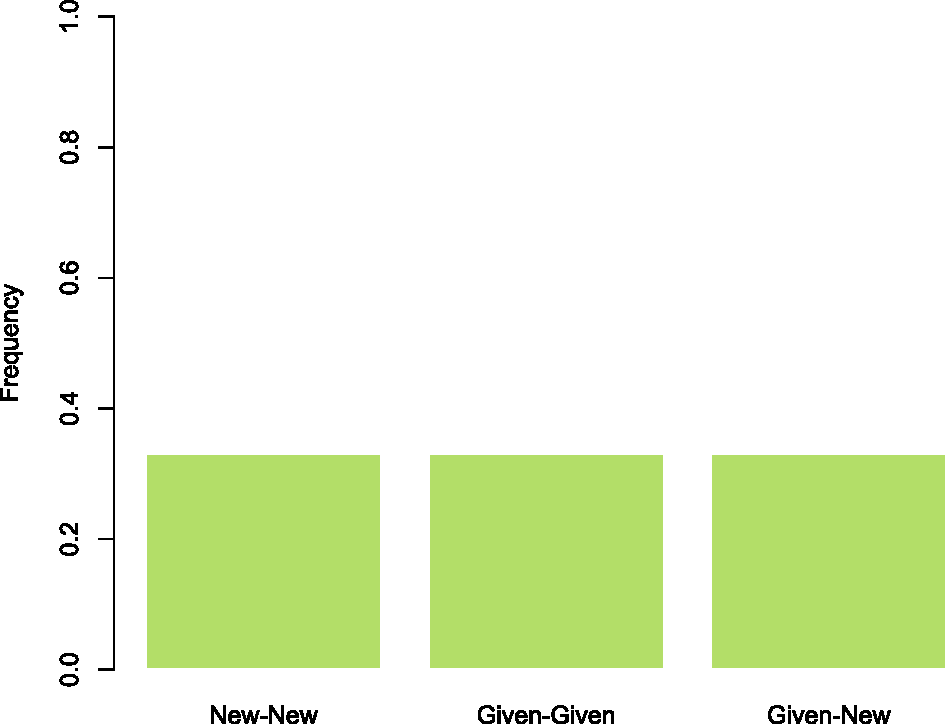
\includegraphics[scale = 0.4]{figures/plotLiteralListenerSbjObjUniform}
\caption{Literal Listener with uniform priors interpreting ``S O''}\label{figure:uniform1}
\end{figure}

A Pragmatic Speaker model generates inferences about what constituent orders a speaker is likely to use in order to convey a certain target information state given the assumptions of the Literal Listener and with the goal of maximizing the chances for the target state to be recovered. Figures \ref{figure:uniform2}--\ref{figure:uniform4} illustrate the inferences of the Pragmatic Speaker with regard to the Given $\succ$ Given, Given $\succ$ New, and New $\succ$ New states, respectively. For instance, the model predicts that in order to convey Given $\succ$ Given a speaker is most likely to use the order ``{\sc det} S {\sc det} O'' or ``{\sc det} O {\sc det} S''. If we look again at table \ref{table:meanings}, we will see that among all the seven configurations eligible to convey a given Given $\succ$ Given information flow, these two are the least ambiguous in that they are associated with only one information state.

\begin{figure}[H]
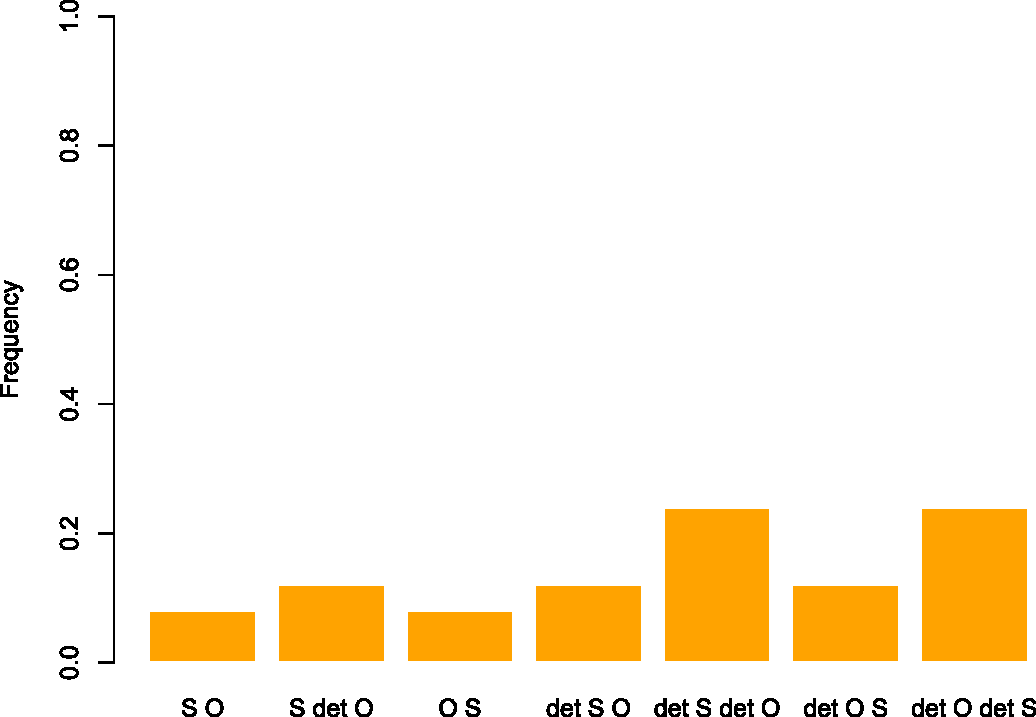
\includegraphics[scale = 0.45]{figures/plotPragmaticSpeakerGivenGivenUniform}
\caption{\small Pragmatic Speaker with uniform priors conveying Given $\succ$ Given}\label{figure:uniform2}
\end{figure}

\begin{figure}[H]
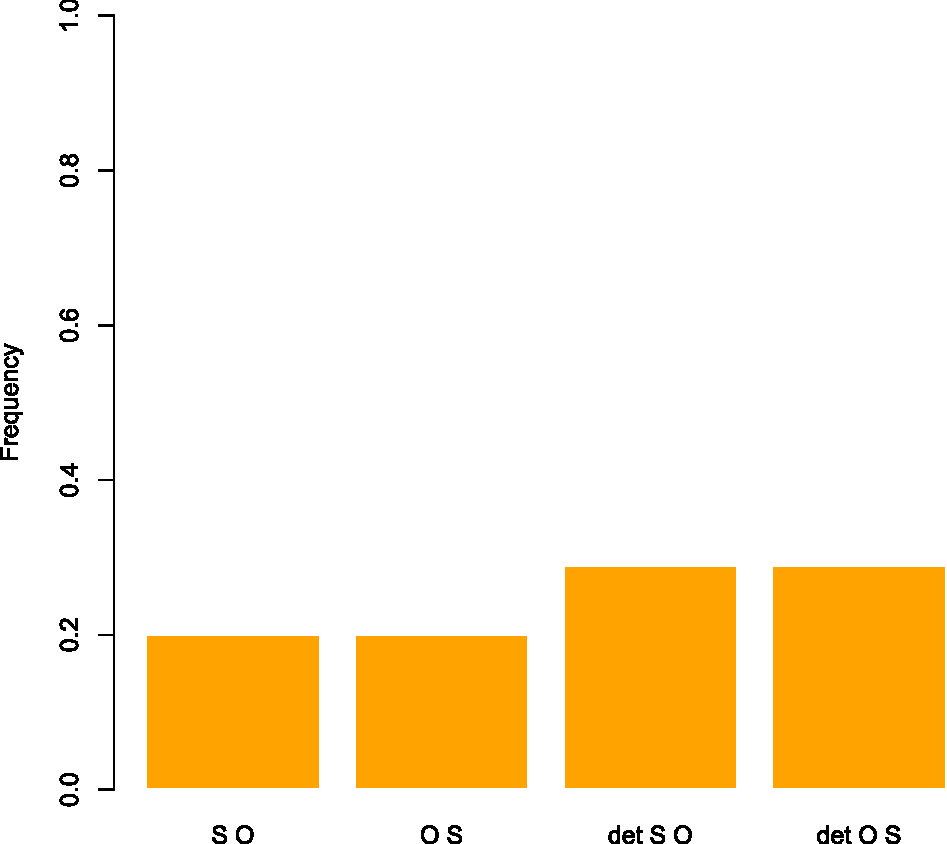
\includegraphics[scale = 0.45]{figures/plotPragmaticSpeakerGivenNewUniform}
\caption{Pragmatic Speaker with uniform priors conveying Given $\succ$ New}\label{figure:uniform3}
\end{figure}

\begin{figure}[H]
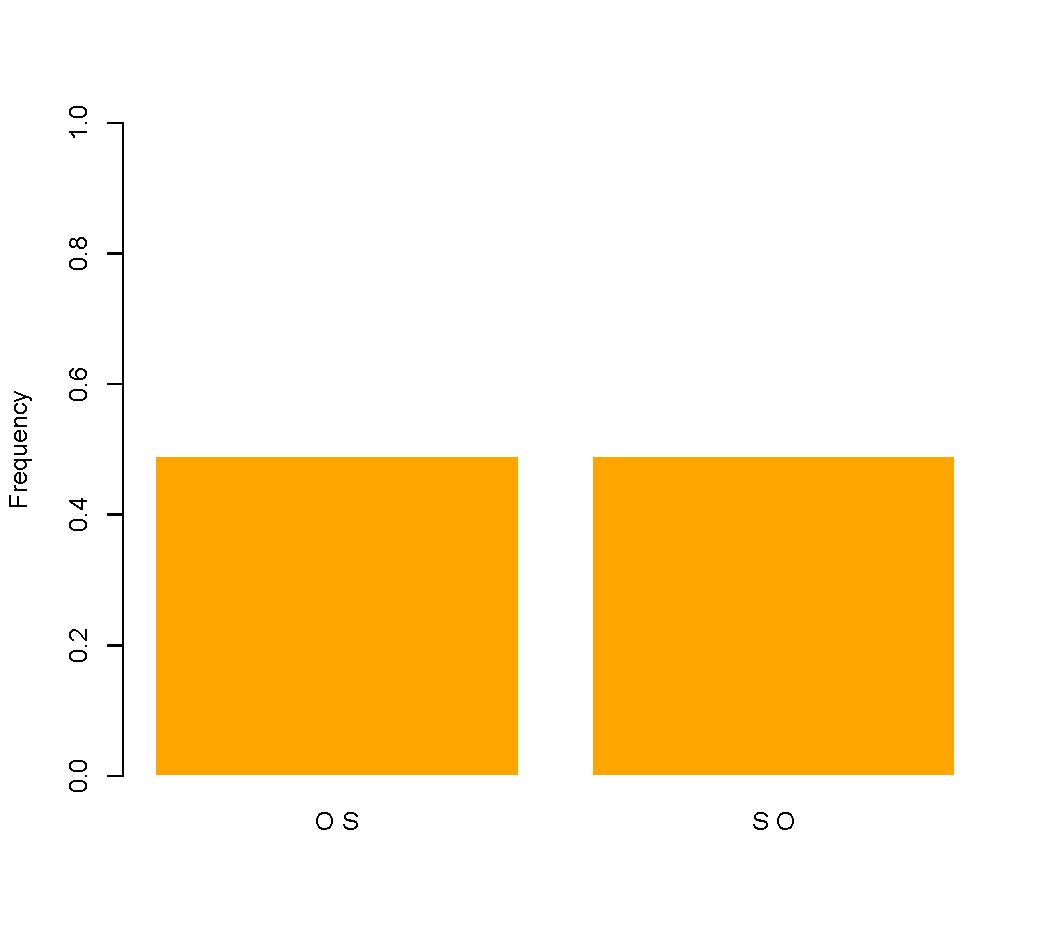
\includegraphics[scale = 0.45]{figures/plotPragmaticSpeakerNewNewUniform}
\caption{Pragmatic Speaker with uniform priors conveying New $\succ$ New}\label{figure:uniform4}
\end{figure}

The New $\succ$ Given state can only be conveyed by one configuration, S {\sc det} O (O {\sc det} S order is not attested in the corpus and therefore is not part of our model).

A model of a Pragmatic Listener involves inferences with respect to the performance of a Pragmatic Speaker. That is, given a particular constituent order, this model makes inferences about most likely interpretations. Inferences for the ``S O'' configuration are shown in figure \ref{figure:uniform5} .

\begin{figure}[H]
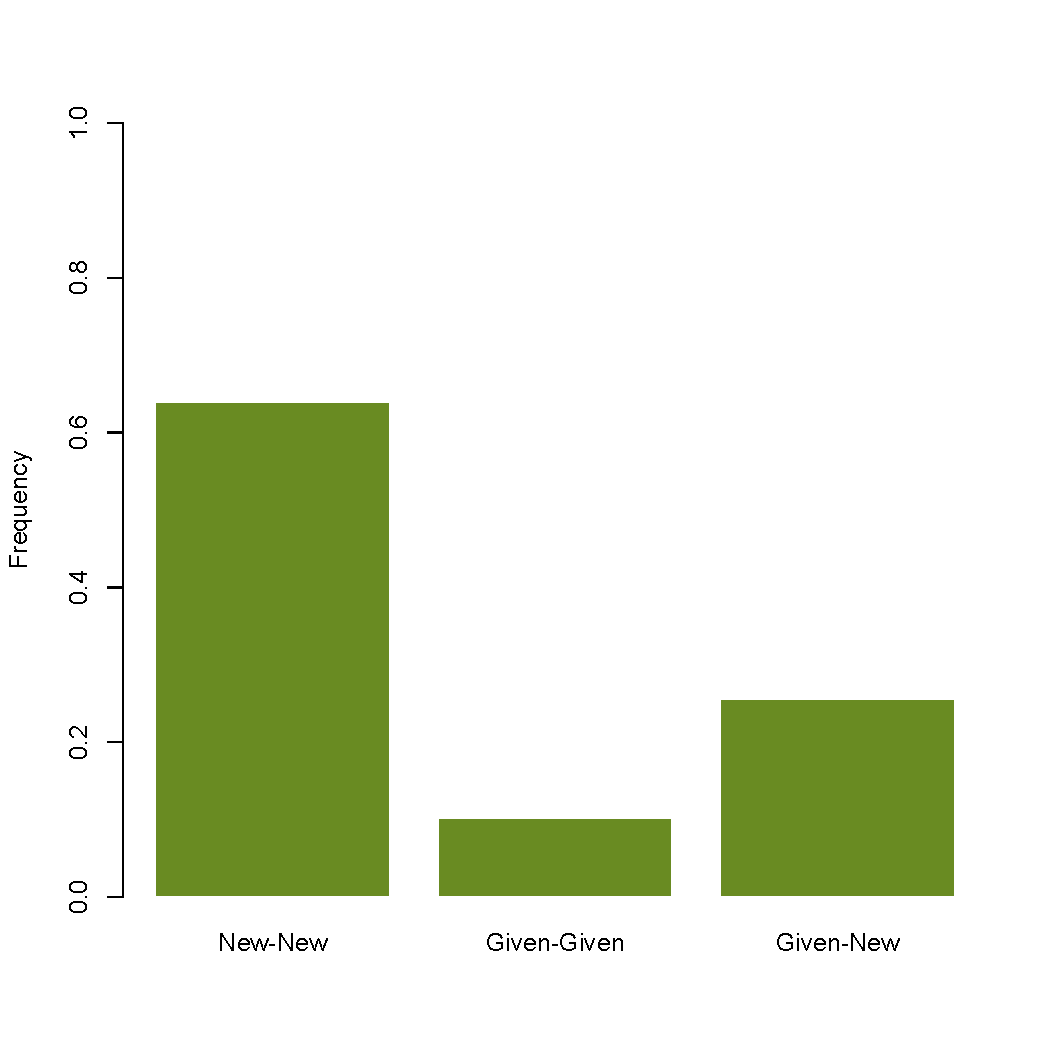
\includegraphics[scale = 0.45]{figures/plotPragmaticListenerSbjObjUniform}
\caption{Pragmatic Listener with uniform priors interpreting ``S O''}\label{figure:uniform5}
\end{figure}

We see that a Pragmatic Listener model predicts that ``S O'' configuration is most likely interpreted as conveying a New $\succ$ New information state. As figures \ref{figure:uniform2}--\ref{figure:uniform4} show, to convey Given $\succ$ Given or Given $\succ$ New, there are better candidates than ``S O'', namely, ``{\sc det} S {\sc det} O'' or ``{\sc det} O {\sc det} S'' and ``{\sc det} S O'' or ``{\sc det} O S'', respectively. That the model predicts ``S O'' to be most likely interpreted as New $\succ$ New corresponds to our intuition that the listener expects the speaker to use ``{\sc det} S {\sc det} O'' or ``{\sc det} O {\sc det} S'' and ``{\sc det} S O'' or ``{\sc det} O S'' for conveying the two other possible states. Since the Speaker visibly did not use either of those, the most likely interpretation is New $\succ$ New, for which there is no better option than ``S O''.

Let us now see how the Pragmatic Listener model fares compared to the historical French data. We classified all bare noun ``S O'' configurations in the corpus as New $\succ$ New, New $\succ$ Given or Given $\succ$ New (recall that we did not find any bare noun ``S O'' corresponding to New $\succ$ Given information state). Figure \ref{figure:corpusSbjObj} shows the distribution of information states among ``S O'' sequences in the corpus.

\begin{figure}[H]
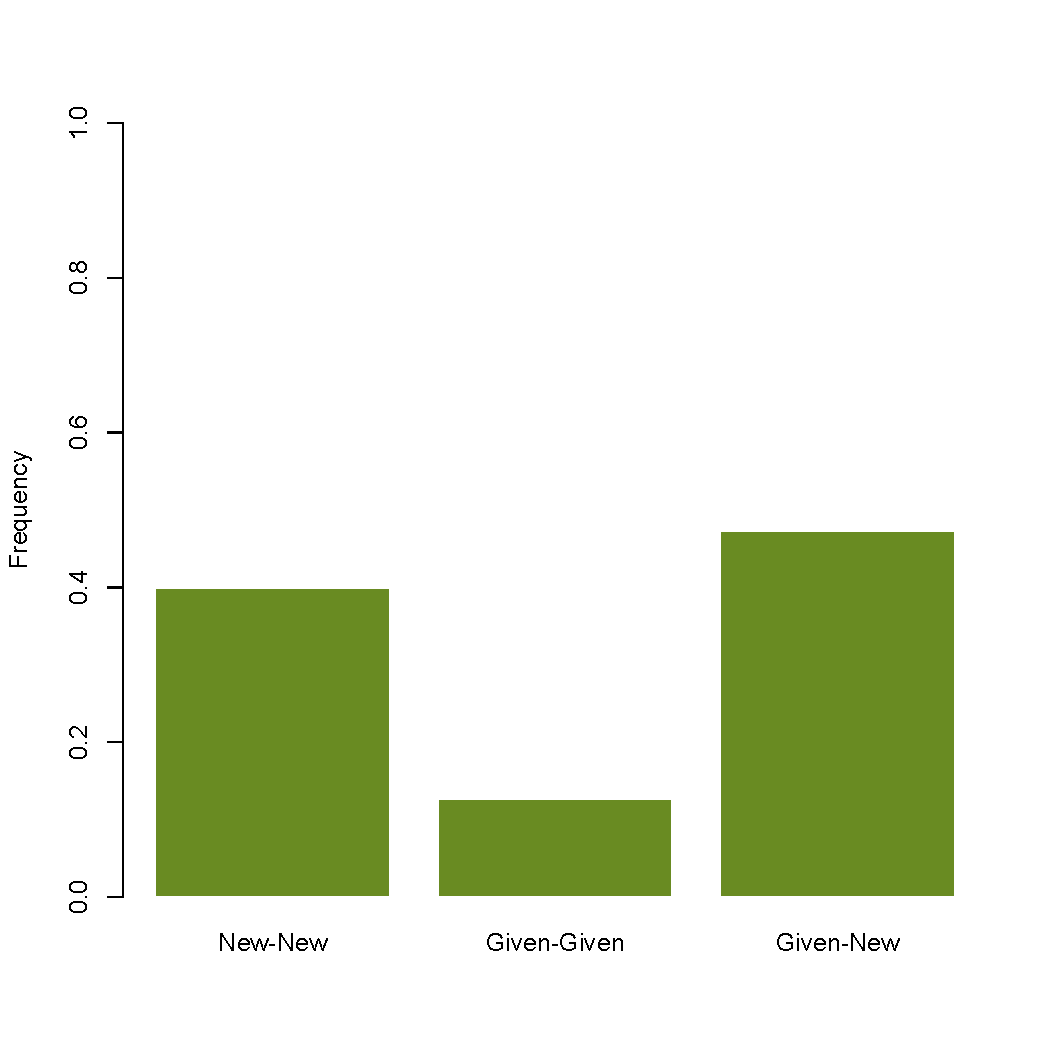
\includegraphics[scale = 0.45]{figures/plotFrenchSbjObj}
\caption{Distribution of informations states among ``S O'' in French, X-XVI c.}\label{figure:corpusSbjObj}
\end{figure}

Comparing these results with the predictions of our RSA Pragmatic Listener model in figure \ref{figure:uniform5}, we see that in the actual data the frequency of Given $\succ$ New is higher than predicted, while the frequency of New $\succ$ New is lower. 

Now, in our model we assumed that apriori all information states are equally likely (they had uniform priors). This is, however, most likely not the case (see \citet{Birner:2012} for references). We therefore need to make our information state priors more realistic. In order to do that, we used data from a syntactically annotated subcorpus of the Russian National Corpus, \citet{RNC}. We classified 430 Russian transitive sentences with bare (i.e. without demonstrative or possessive determiners) nominal arguments (both ``S O'' and ``O S'') according to their information state. The obtained distribution is plotted in figure \ref{figure:Russian}.

\begin{figure}[H]
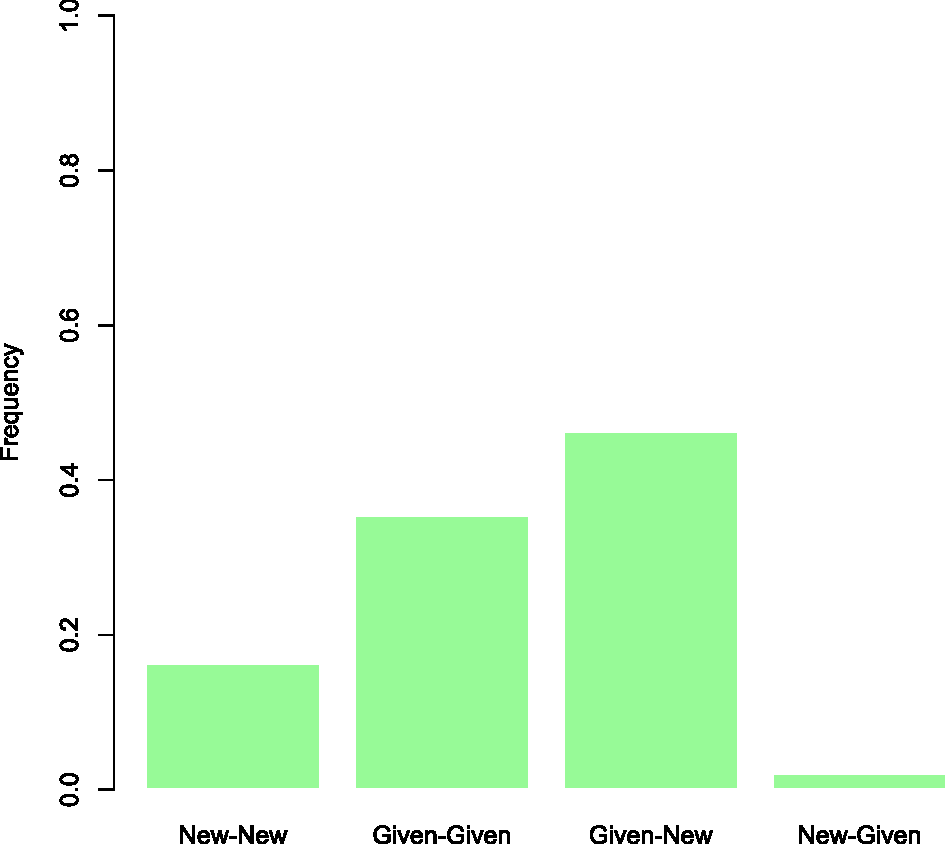
\includegraphics[scale = 0.45]{figures/plotRussianSbjObj}
\caption{Distribution of informations states among transitive clauses with bare nominal arguments in the Russian National Corpus}\label{figure:Russian}
\end{figure}

We used these frequencies to set the priors for the information states in our RSA model. That is, instead of assuming that information states Given $\succ$ Given, Given $\succ$ New, New $\succ$ Given, and New $\succ$ New are equally likely, we set their probabilities to 0.35, 0.46, 0.02, and 0.16, respectively. We then reran our Pragmatic Listener model, which now generates inferences for interpreting ``S O'' configuration as in figure \ref{figure:models}, where it is plotted against the historical French data.

\begin{figure}[H]
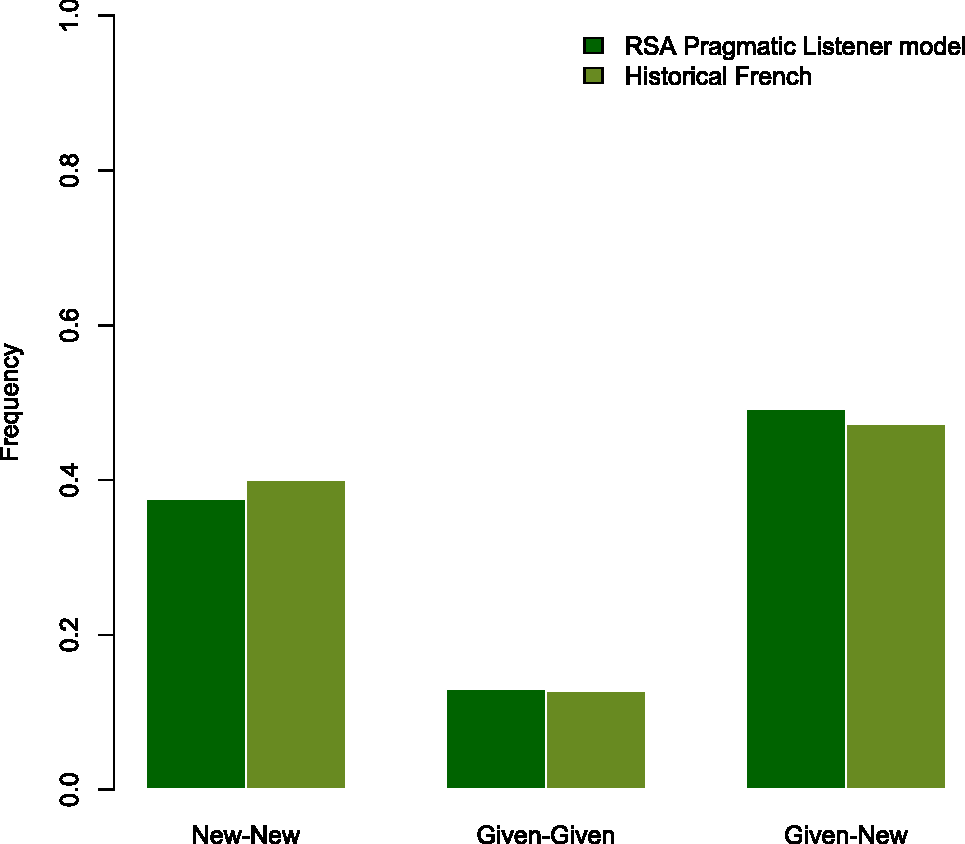
\includegraphics[scale = 0.45]{figures/plotModelComparison}
\caption{Distribution of informations states among ``S O'' as predicted by Pragmatic Listener model and in historical French corpus}\label{figure:models}
\end{figure}

As the figure shows, the shapes of the two distributions are remarkably similar, which means that our RSA Pragmatic Listener is a successful simulation of the pragmatic reasoning behind the historical French data. 

The core assumptions of the simulation are encoded in the morphological entries in table \ref{table:meanings}, where the strings with presupposition-triggering determiners are less ambiguous than strings with bare NPs only and where New $\succ$ Given information state cannot be conveyed by utterances involving bare nouns. This has the effect of predicting that, first, whenever there is a choice, speakers will be more likely to use strings with determiners than strings without, as this maximizes their chance to be understood (see figures \ref{figure:uniform2} and \ref{figure:uniform3}), and, second, that pragmatically reasoning listeners will tend to interpret bare nouns as conveying information states which could not have been conveyed using presupposition-triggering determiners, such as New $\succ$ New (see figure \ref{figure:uniform5}). The simulation results match historical French data very closely, while they contrast with the data we took from the Russian National Corpus where Given $\succ$ Given is the second frequent information state of a transitive clause with bare nouns (see figure \ref{figure:Russian}). We suggest that the differences is due precisely to the lack of definite determiners in Russian, which means that there is no better alternative for conveying Given $\succ$ Given than bare NPs, while in French ``{\sc det} S {\sc det} O'' is the best option (see figure \ref{figure:uniform2}). 

\section{Givenness marking and constituent order frequencies}
\label{section:orders}

In this section, we explore a connection between givenness marking and constituent order frequencies in historical French. Let us take another look at the constituent order distribution in table \ref{table:orders}. Orders involving O $\succ$ S are markedly more rare than those with S $\succ$ O, with one exception, namely, the OVS configuration. First, we suggest that the rarity of O $\succ$ S in medieval French, and thus the rarity of OSV and VOS, is a consequence of \#New $\succ$ Given on the assumption that subjects denote given information more frequently than objects. This assumption can be tested, at least at a first approximation, by looking at the distribution of determiners with subjects and objects. The rates of definite and possessive determiners and demonstratives with subjects and objects will be indicative of their respective tendencies to be associated with existential presupposition. Figure \ref{figure:determiners} shows the determiner distribution with subjects and objects per century.

\begin{figure}[H]
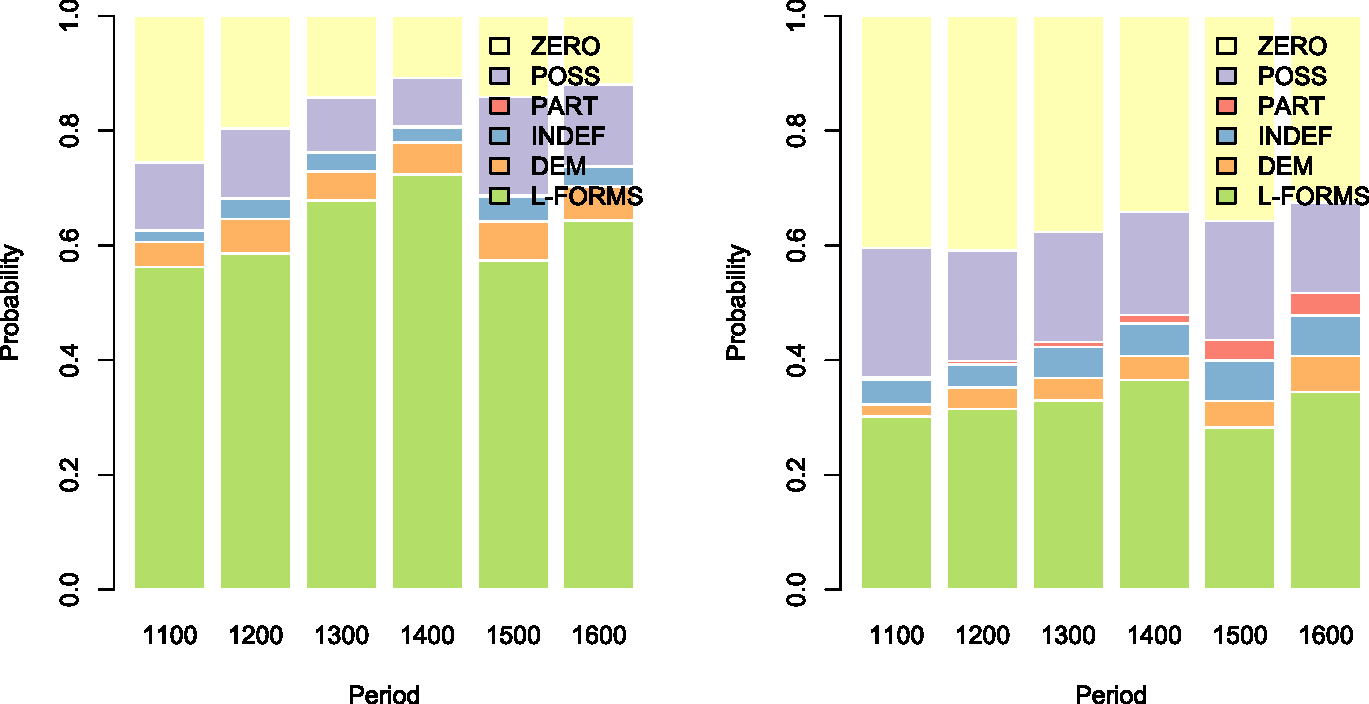
\includegraphics[scale = 0.45]{figures/determiners.pdf}
\caption{Determiner distribution: subjects vs. objects}\label{figure:determiners}
\end{figure}

Based on this approximation, we can estimate that during all periods subjects are at least 2--3 times more likely than objects to occur with a definite, possessive or demonstrative determiner, which indicates that subjects are much more likely to satisfy the conditions on the use of presupposition-triggering determiners, namely, to denote an individual whose existence is entailed by the Common Ground. 

Extrapolating this conclusion onto clauses with bare arguments, we expect that subject noun phrases denote properties whose extension is entailed by the Common Ground to be non-empty much more frequently than objects. This, in turn, means that the order S $\succ$ O is expected to align with the (licit) information state Given $\succ$ New much more frequently than the order O $\succ$ S. We suggest that this is at least in part responsible for the very low frequency of OSV and VOS orders in historical French.\footnote{According to \citet{wals-81}, in a sample of 1188 languages where a dominant constituent order can be established, there are only 40 languages (or $\approx$ 3\%) where the dominant order involves O $\succ$ S.}

We also observe that OVS order is more frequent than OSV and VOS. We suggest that OVS corresponds to a configuration of topic (situation) shift, where the preverbal position is associated with prosodic prominence. To probe into the properties of OVS, in figure \ref{figure:determinersOrders} we plotted distributions of determiners in the object position in finite clauses with different constituent order. We take all the clauses with nominal objects and any type of subject (i.e. either nominal or pronominal or null). 

\begin{figure}[H]
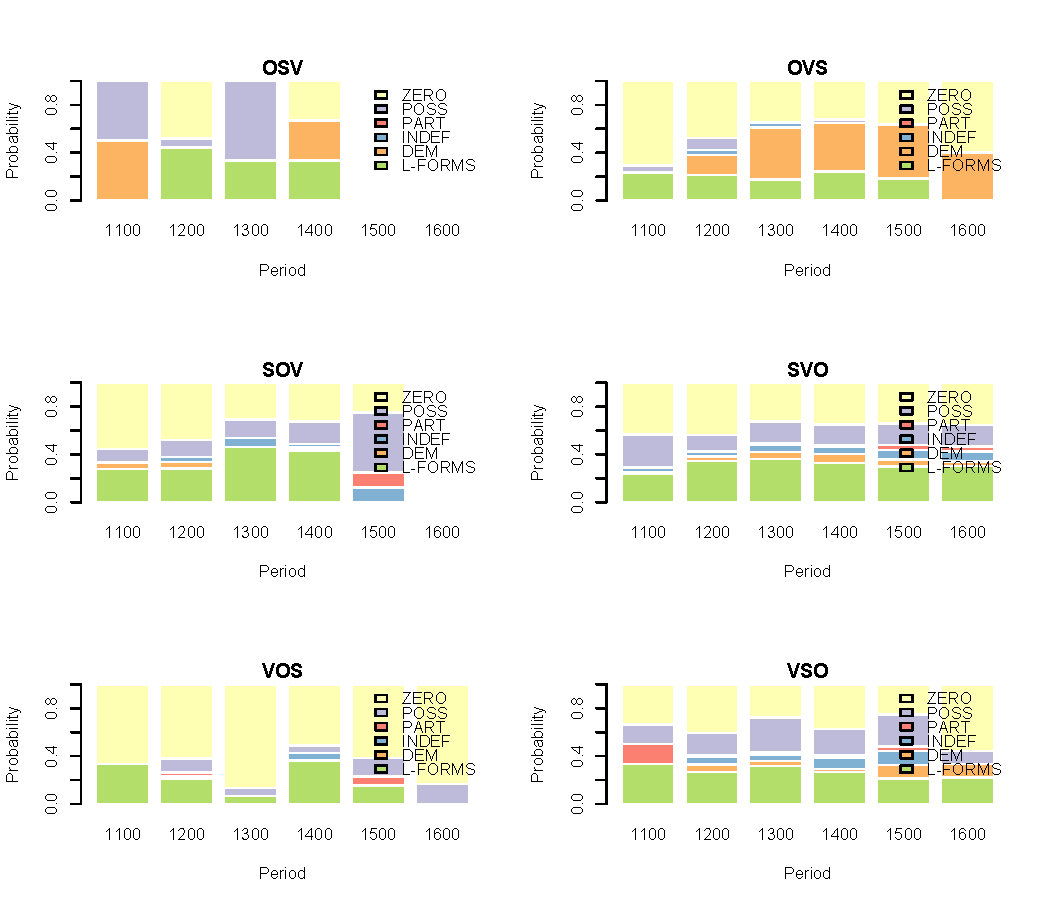
\includegraphics[scale = 0.55]{figures/determinersOrders.pdf}
\caption{Determiner distribution in object position}\label{figure:determinersOrders}
\end{figure}

%This is in line with an independently attested series of developments which consisted first in the spread of the {\it le}/{\it la}/{\it les} determiners, somewhat later of {\it un}/{\it une} determiners, and, finally, of the {\it des} determiners. The spread of these forms was presumably accompanied by their reanalysis from demonstratives, numerals and partitive determiners into definite and indefinite ones (\citealt{Carlier:2001}, \citealt{Carlier:2007b}, \citealt{MulderCarlier:2011}). %ADD references

Excluding from consideration numerically marginal (see table \ref{table:orders}) and therefore highly erratic OSV and VOS patterns, we observe a similarity between object determiner distributions in SOV, SVO, and VSO configurations. 

%OSV and VOS are characterized by the lowest and the highest rates of bare nouns, respectively. An example of an OSV clause with a bare object is given in (\ref{osvBare}). There are 125 finite OSV clauses with a nominal object and an overt subject (either nominal or pronominal).

%\ea
%\gll mortal poison$_{obj}$ la dame$_{sbj}$ boit\\
%deadly poison det lady drinks\\
%\glt ``the lady drinks a deadly poison'' \hfill \scriptsize{(1155-ENEAS1-BFM-R,25.519)} \label{osvBare}
%\z

%The low rate of bare nouns in the object position OSV is expected given the conclusion reached above that subjects are very likely to be given (based on the rate of definite determiners) and that an OSV order with a bare and therefore possibly non-given object would violate *New $\succ$ Given.

%Most cases of VOS with bare objects involve nouns which can be considered as forming a complex predicate with the verb and are thus exempt from *New $\succ$ Given (e.g. \ref{vosBare}). 

OVS stands out by an exceptionally high proportion of demonstratives in object position. To understand what that means for the status of OVS, let us consider the role of demonstratives in the information structure in modern languages. 

The most notable feature of demonstratives is the requirement to have an antecedent (or an element in the extralinguistic reality serving as a referent). This property has been captured by assuming a silent individual pronoun in the structure of demonstrative phrases (\citealt{Nunberg:1993}, \citealt{Elbourne:2008}). On the view that pronominals are variables which get their value based on a context-determined mapping, in order for such structure to be interpretable, the context must involve a salient individual to which the assignment function will map the pronominal index. 

%	\item[] {\scriptsize silent pronouns do not carry $\phi$-features, which have been argued to facilitate long-distance anaphora (e.g. \citealt{Dillon:2015} for Chinese anaphors);} %This means that noun phrases with demonstratives, if interpretable, will necessarily denote an individual whose existence is entailed by the Common Ground.

Another potentially relevant fact is that the antecedent of a demonstrative is normally available in the immediately preceding context. According to \citet[180]{Zulaica:2011}, in Spanish, 80\% of demonstratives have their antecedents in the immediately preceding utterance. \citet[204]{StevensLight:2013} report that in English 78.08\% of demonstratives have antecedents that are discourse-new in the context immediately preceding the relevant demonstrative.

In addition, demonstratives, in contrast to definite determiners, are characterized by the requirement that the nominal predicate do not denote a singleton (relative to a certain domain, \citet{Corblin:1987}). This is illustrated by the infelicity of (\ref{dem1}) and (\ref{dem2}) with demonstratives in the contexts implying uniqueness and by their felicity in contexts involving more than one individual with the relevant nominal property, as in (\ref{dem3}).

\ea
I fed \#that/the dog. (If the speaker owns just one dog.)\label{dem1}
\z

\ea
I saw \#that/the brightest star.\label{dem2}
\z

\ea
 A woman$_{i}$ entered from stage left. Another woman$_{j}$ entered from stage right. That/\#the woman$_{j}$ was carrying a basket of flowers. \label{dem3} \hfill (From \citealt{Roberts:2002} \& \citealt[74]{Wolter:2006})
 \z

These three facts mean that an object noun phrase with a demonstrative requires an immediately preceding antecedent and that it also requires that the extension of the nominal predicate in the relevant situation do not correspond to a unique entity. An antecedent for a demonstrative must introduces a new entity, since an entity which had been introduced before would normally be realized as a pronoun or a noun phrase with a definite determiner, which is incompatible with the non-uniqueness requirement. In this respect, consider examples in (\ref{dem4}) and (\ref{dem5}).

%Here there may be a requirement that the noun phrase is also mentioned, just a pronominal is not enough. Or the newness requirement is a kind of economy condition, why use the demonstrative 
%Presumably after a pronominal mention it is uneconominal to use a demonstrative DP which invokes a noun again.

\ea
Workers painted a house$_{new}$. That house really needed it.\label{dem4}
\z

\ea
Workers painted the house/it$_{old}$. \#That house really needed it.\label{dem5}
\z

%Is there also a novelty requirement for demonstratives?	It can be derived from anti-uniqueness presumably

Based on such considerations, \citet{BoschEtAl:2003} formulate a Complementary Hypothesis, which states that personal pronouns pick up discourse topics as referents, while demonstratives prefer non-topical referents. Furthermore, \citet[175]{Zulaica:2011} argues for Spanish that ``speakers use demonstratives to mark topic or subtopic shifts''. We thus conclude that the high rate of demonstratives with objects in OVS configurations indicates that the preverbal position was frequently used to indicate a shift in topic situation. %While we are not ready to give a proper definition of the relevant topic situation shift here, we speculate that it can be conceived of as a change in the restrictor of QUD. 
	
% assuming its resource situation becomes a topic situation wrt which the whole proposition is evaluated (\citealt{Kratzer:1989}, \citealt{Elbourne:2008}, \citealt{Schwarz:2009}).

%\begin{figure}[H]
%\centering
%\begin{tikzpicture}[sibling distance=-5pt]\scriptsize
%\tikzset{level distance=25pt}
%\Tree [.TopP [.{\bf Object} ] [.TopP [. Top ] [.AgrP [.{\bf V}-T-Agr ] [.TP [.{\bf Subject} ] [.TP [.$<$V-T$>$ ] [ .... ] ] ] ] ] ] 
%\end{tikzpicture}
%\caption{OVS in Medieval French}\label{fig:ovs}
%\end{figure}

%The reason of the encroachment onto the territory of bare nouns is less clear. We suggest that it is related to the prosodic reorganization that took place in Medieval French, as a result of which the preverbal position lost its prominence. \citet[216]{Rainsford:2011} argues for Old French based on metrical considerations that ``XP constituents moved to CP [the preverbal position -- Authors] are realized as stressed'' and that this phenomenon ends up disappearing. It has been argued that prosodic prominence, such as primary stress, indicates topic shift in the case of topical constituents with given referents (\citealt[325]{Lambrecht:1996}). According to \citet{Buring:2003}, in English contrastive topic is realized by a fall-rise accent.

%cited from Francisco Ocampo https://books.google.be/books?id=afUFtOc0KekC&pg=PT218&lpg=PT218&dq=topic+shift+stressed+prosody&source=bl&ots=G3kt7emVnb&sig=_OoEZH2B1tHtrVfL3IQ6wrSFr8s&hl=en&sa=X&ved=0ahUKEwjJ8aHpvfbbAhXFaFAKHTHtBZM4ChDoAQgoMAA#v=onepage&q&f=false

%\item{\small \citet[61]{LabelleHirschbuhler:2005}: the initial constituent may be either topicalized or focalized.}
%\item{\small \citet{Kroch:1989} \& \citet{Rainsford:2011}: it was the change in the prosodic organization of French which caused the V2 grammar to die out.}
%In the larger perspective, this supports the claim that prosody can cue syntactic analysis (Fatima Hamlaoui's talk yesterday) \& drive language change.

%\item \citet{LabelleHirschbuhler:2005}: disappearance of a discourse-oriented left-peripheral projection;
%\item \citet{Vennemann:1974}, \citet{Harris:1978}, \citet[100]{MarchelloNizia:1995}: passage from Topic-initial to Subject-initial structure.

\section{Conclusions} 
\label{section:conclusions}

%ADD ADD The rise of discouse-new complements in preverbal position found in Larrivee may be related to the rise of morphological markers which obviate the *New > Given

%ADD invoke disappearing prosody as a factor which used to make constituent order a more efficient signal

In this paper we explored organization of the information in a clause in light of Ku\v{c}erova's (2012) proposal that givenness, when not expressed by dedicated morphemes, is monotonically marked from left to right. We proposed an amended version of the constraint that involves a non-presuppositional existential inference as the definition of givenness and tested it on a historical corpus of French, since the historical stages of French have both syntactic and morphological means of marking givenness. Our results show that the principle is borne out in the French historical data: in a corpus of 1,5 million words, we did not find any cases of New $\succ$ Given in clauses with bare arguments. The data also bear out the prediction that in case Given is marked morphologically, the left-to-right monotonicity requirement does not apply.

We also built the principle into a game-theoretic simulation of the use of constituent order and presupposition-triggering determiners to convey an information state. The results of our simulation come very close to the empirical historical French data, suggesting that it is viable component of a model of pragmatic language use. 

Finally, we also showed that *New $\succ$ Given may provide insight into relative frequencies of various constituent orders.

\section*{Abbreviations}
\section*{Acknowledgements}

{\sloppy
\printbibliography[heading=subbibliography,notkeyword=this]
}
\end{document}
